\chapter{\label{ch:chargeid}Charge Identification with Convolutional Neural 
Networks} 

\minitoc

The correct categorisation of particle interactions in the detector is a major
problem faced by any particle physics experiment. This typically starts with
identifying low level features of the interactions, which can then be used to
gradually build up a picture of the full interaction. In DUNE, the
classification of neutrino interactions requires identifying the lepton content
of the final state, and in \protodune{}, cross section analyses rely on
accurately identifying the particles in the interaction. Therefore, it is
important to be able to distinguish muons and pions from electrons in LArTPCs, 
or more generally, tracks from showers.

In order to build up a complete picture of an event, it is useful to begin by
identifying the small features of the interaction, which can then be used to
gradually build an understanding of the full event. In \protodune{}, the
smallest reconstructed features are the hits, which correspond to small charge 
depositions collected on individual wires. Classifying these hits provides
useful information for future analyses, and can potentially be used to aid
decision making during event reconstruction.

This chapter will describe an approach to hit classification in LArTPCs using
machine learning techniques. Section \ref{hit-id} will detail an approach to 
hit classification in LArTPCs based on identifying the source of energy 
depositions with a convolutional neural network.  The performance of this 
approach will be analysed with ProtoDUNE--SP simulation and data in sections 
\ref{cnn-perf-sim} and \ref{cnn-perf-data} respectively.

\section{Hit Identification with Convolutional Neural Networks} \label{hit-id}

Effective track shower separation forms the basis of many reconstruction
challenges in DUNE and \protodune{}; it needed to define pure calibration
samples, such as minimum ionising muons and $\pi^0$ decays, and it is an
important part of neutrino event reconstruction. Each event sample leaves a
unique signature in the detector, but the first step in reconstructing these
samples is the same, reconstructing tracks and showers which can be combined to
build the final state. 

In a LArTPC, tracks and showers are built from collections of hits, these hits
have to be clustered and identified as track or shower objects. In this section,
we will describe a method for identifying the source of hits in the \protodune{}
LArTPC. The classification of each hit is stored as part of the reconstructed
output in LArSoft, and can be used by subsequent reconstruction and analysis
algorithms.

As well as track and shower objects, Michel electrons are a useful calibration
sample in LArTPCs. Michel electrons are electrons produced when a muon decays at
rest, which have an energy spectrum in the range of 1--50 MeV. As discussed in 
Chapter \ref{ch:energyloss}, the critical energy for electrons in liquid argon
is at around 30 MeV. Therefore, Michel electrons have a unique signature in
LArTPCs, and they were included as a unique category in the classification
algorithm.

\subsection{Data Preparation}

A CNN was designed for the hit classification, the network was trained to
predict,
\begin{equation*}
	\left[ p_t, p_s, p_e \right] \mbox{ and } \left[ p_m \right]
\end{equation*}
where $p_t$, $p_s$, $p_e$, and $p_m$, are the probabilities for track, shower,
empty, and Michel electron classifications respectively. The empty category is
included to ensure that the network doesn't learn to assign track--like or
shower--like classifications to empty or noisy regions of the data. In addition,
because the Michel electron category has an overlap with the track and shower
categories, the Michel electron probability is decoupled from the other
probabilities. The track, shower, and empty (TSE) probabilities are 
constrained to sum to one, such that every hit is classified into one of these 
categories.

An input image was produced for every reconstructed hit, the hit being
classified is at the centre of the image. These images were produced from the 
wire readout data, after the noise removal and 2D deconvolution steps 
described in Chapter \ref{ch:protodune}. Each input image is $48 \times 48$
pixels, with each pixel being filled with the ADC value from the wire readout
data, variations in wire to wire response and gain are applied before building
the images. The width of the image corresponds to one wire per pixel, and the 
height is the time coordinate. The time data is downsampled, using an average 
over time samples, such that the spatial dimensions of the image are the same 
in both directions. Therefore, each image represents around $24 \times 24 
\mbox{ cm}^2$ of wire data. Examples of an input image from each none empty 
class are shown in Figure \ref{fig:patches}, which also demonstrates the 
relationship between the images and the detector readout.

\begin{figure}
	\centering
	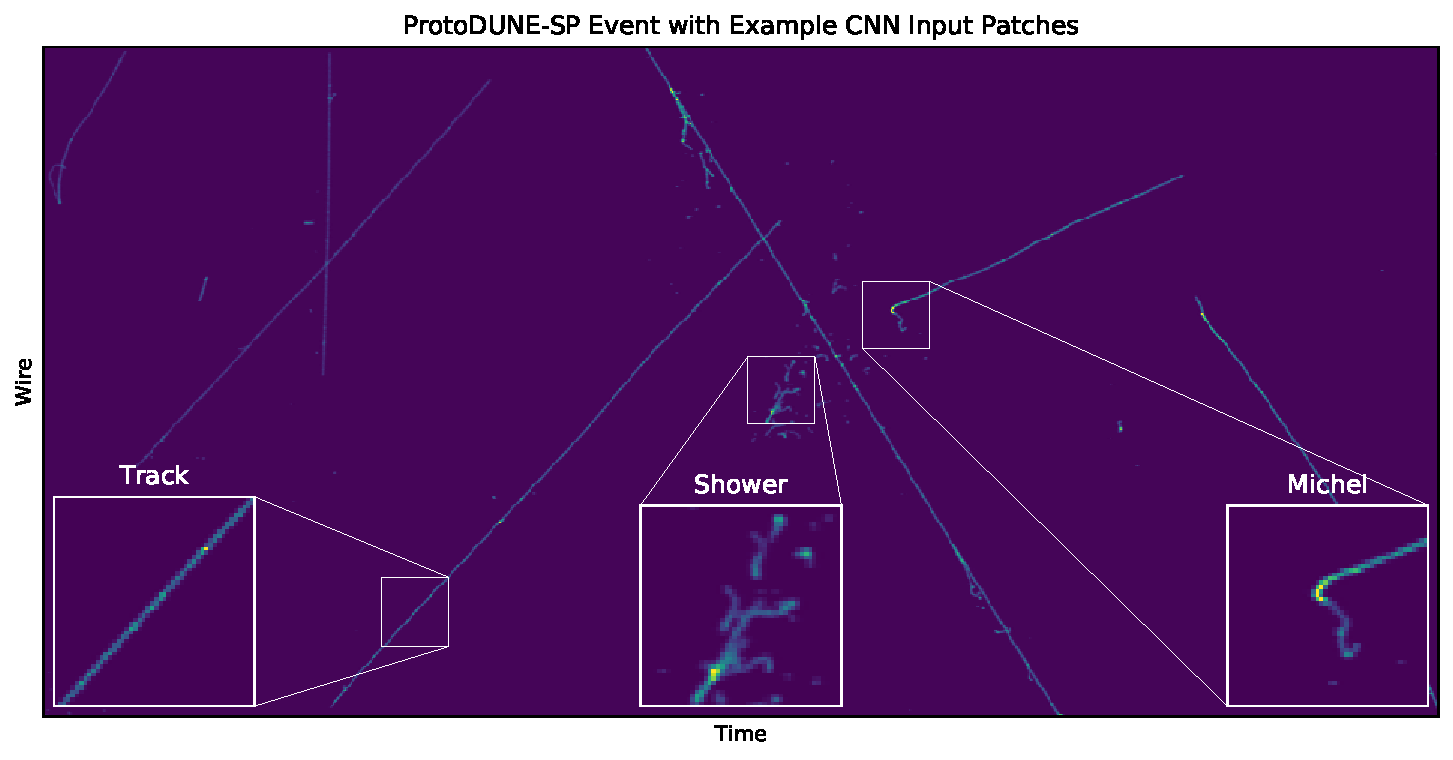
\includegraphics[width=\textwidth]{figures/patch_zoom.pdf}  
	\caption
	[Example CNN input images for each class.]
	{Example CNN input images for each class.}
	\label{fig:patches}
\end{figure}

The true classification for each sample was obtained from the simulation, by 
associating the measured ionisation energy depositions to the corresponding
simulated particle. If the reconstructed hit is not associated to a true
particle, then this hit is due to noise and the true classification is empty.
The truth vectors for different true particle sources are detailed in Table
\ref{tab:ground_truth}. \mccorrect{TODO, discuss why.}

\begin{table}
	\centering
	\begin{tabular}{c|c|c}
		Ionisation Source & Track, shower, empty & Michel \\ \hline
		Muons             & [1,0,0]              & [0]    \\
		Hadrons           & [1,0,0]              & [0]    \\
		Michel Electrons  & [0,1,0]              & [1]    \\
		Other Electrons   & [0,1,0]              & [0]    \\
		Noise             & [0,0,1]              & [0]    \\
	\end{tabular}
	\caption
	[Truth labels for different particles.]
	{Truth labels for different particles.}
	\label{tab:ground_truth}
\end{table}

The training data for the CNN was built using simulations of the \protodune{}
detector in the LArSoft framework; the simulations used were under beam
operating conditions, and therefore included simulations of cosmic rays, and
test beam particles in the range of 1--7 GeV. Around 29 million input images
were produced in total for the training, this sample was split into three
datasets, the training, validation, and test sets. The training set is used to
train the CNN, the validation set is used to monitor the performance of the CNN
during training, and the test set is used as an initial verification of the 
performance of the network after training. Details of the number of patches of
each type in these three datasets are detailed in Table \ref{tab:patches}.

\begin{table}
	\centering
	\begin{tabular}{c|c|c|c|c|c}
		Dataset    & Shower     & Track      & Empty     & Michel  & Total      \\ \hline
		Training   & 13,493,982 & 9,727,604  & 2,517,882 & 731,456 & 26,470,925 \\
		Validation & 734,673    & 562,038    & 141,388   & 42,727  & 1,480,826  \\
		Test       & 764,659    & 518,805    & 139,987   & 39,674  & 1,463,125  \\ \hline
		Total      & 14,993,314 & 10,808,447 & 2,799,257 & 813,857 & 29,414,876
	\end{tabular}
	\caption
	[Number of input images with each truth label.]
	{Number of input images with each truth label.}
	\label{tab:patches}
\end{table}

\subsection{Network Architecture}

The network architecture for this CNN was designed to provide the best possible
performance given constraints on running time and memory usage during network
evaluation, when run on CPUs during the \protodune{} reconstruction chain. 
This CNN is part of the low level reconstruction chain for \protodune{}, and 
it's run time is required to be on the order of 10 seconds per event. In 
addition, the CNN should not increase the maximum memory usage during 
reconstruction beyond around 4 GB. There is currently ongoing work looking 
into using GPUs during the network evaluation, which would allow more complex 
architectures to be used, and therefore potentially increase performance.

The network architecture is used is shown in Figure \ref{fig:arch}. The images
are first processed by convolutional layer with 48 $5 \times 5$ filters, this
layer extracts feature maps from the data. The responses from the 
convolutional layer are passed through the Leaky ReLU activation function, which
is discussed in Chapter \ref{ch:ml}, before being processed by the dense 
layers. The feature maps are processed by a pair of dense layers, with 128 and 
32 nodes respectively. These layers also use the Leaky ReLU activation
function. After the second dense layer the network is split into two branches in
order to make it's prediction. The first branch returns the prediction for the 
TSE categories, and the second branch for the Michel electron category. The 
first branch uses a Softmax activation function, which ensures that the scores 
for the TSE categories sum to one.  The second branch uses a Sigmoid 
activation function, which ensures that the Michel electron scores are bounded 
between zero and one. The choice of activation functions in the output layers 
allows for a pseudo--probabilistic interpretation of the scores from the CNN.

\begin{figure}
	\centering
	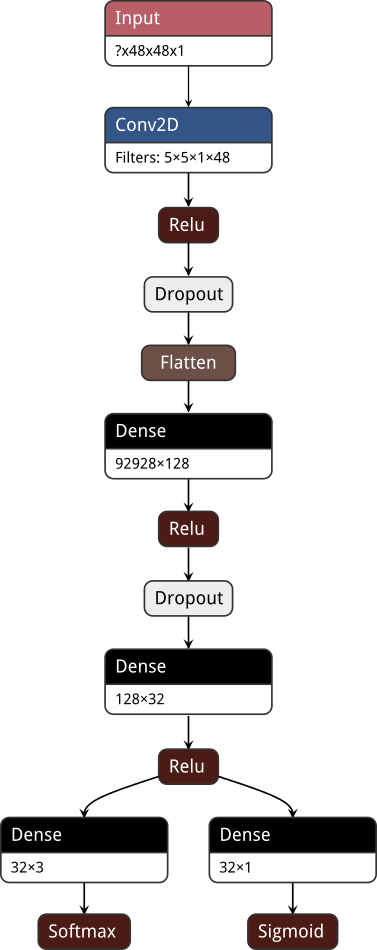
\includegraphics[height=0.7\textheight]{figures/track_shower_arch.png}
	\caption
	[Network architecture used for hit classification.]
	{Network architecture used for hit classification.}
	\label{fig:arch}
\end{figure}

Two dropout layers are used in the network, these layers are used as part of the
regularisation of the network. A dropout probability of 0.5 is used in both of
the dropout layers. The dropout algorithm is discussed in Chapter \ref{ch:ml}.

The loss of the network was the weighted sum of the losses for the two output
branches,
\begin{equation*}
	L = 0.1 \cdot L_{TSE} + L_M,
\end{equation*}
where the Michel electron loss is given higher precedence due to the smaller
training dataset available for the Michel electron output. The loss function for
the TSE branch is the categorical cross entropy 
loss\cite{750fabedbacb467c8fafd98b87f77436}, and for the Michel electron branch
it is the mean squared error\cite{mse_springer},
\begin{align*}
	L_{TSE} &= - \frac{1}{N} \sum_{j=1}^N \sum_{i=0}^2 (t_j)_i \log (p_j)_i, \\
	L_M &= \frac{1}{N} \sum_{j=1}^N (t_j - p_j)^2
\end{align*}
where $t_j$ and $p_j$ are the truth and the prediction for the $j$ sample in the
training batch, and $i$ sums over all outputs in the TSE branch.
\mccorrect{TODO, explain choices.}

\subsection{Training and Validation}

The TensorFlow\cite{45381} library and the Keras\cite{chollet2015keras} 
application programming interface (API) were used to design and train the CNN, 
which was trained on a dedicated \protodune{} server at CERN, with an NVIDIA 
GTX 1080 GPU. The training was monitored using the TensorBoard visualisation 
toolkit, which is part of the TensorFlow library. 

\mccorrect{TODO, maybe move the in depth discussion to the NN chapter}
The CNN was trained using the stochastic gradient descent (SGD)
algorithm, including both the momentum and decay 
algorithms\cite{Reed1999}. The momentum algorithm reduces the oscillations of
the weights during learning, while the decay of the learning rate allows for
rapid learning during early stages of SGD, and increased precision as the model
converges. 

During training the learning metrics where monitored with TensorBoard. The
losses for each branch and the total loss were monitored for the training
and validation datasets. The validation loss was calculated once per training
epoch, which is one iteration through the full training dataset, and the
training loss is averaged at the end of each epoch. The training and validation
losses as a function of training epoch are shown in Figure \ref{fig:training}.
The weights of the network were saved at the end of each epoch. The final
weights were chosen based on the early stopping algorithm discussed in Chapter
\ref{ch:ml}, focussing on the TSE branch of the network, this is highlighted 
in Figure \ref{fig:training}.

\begin{figure}
	\centering
	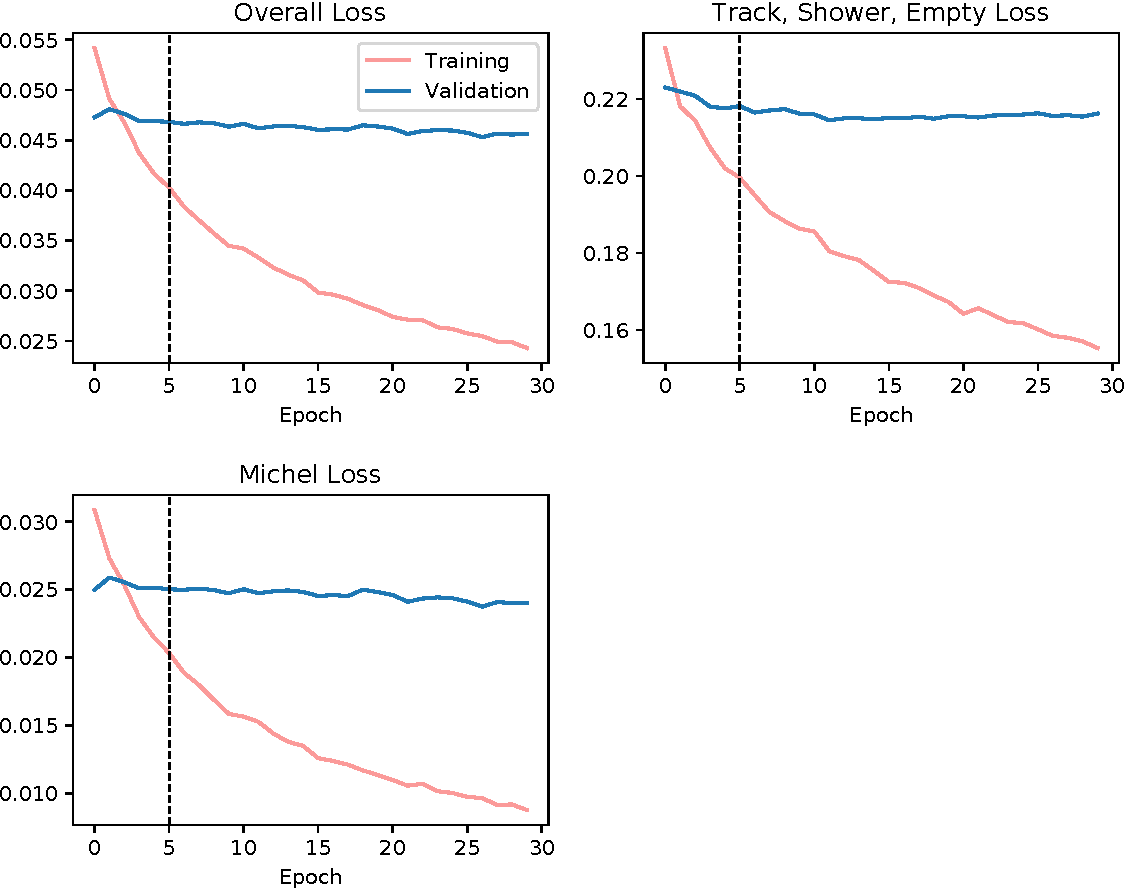
\includegraphics[width=\textwidth]{figures/losses_prelu.pdf}
	\caption
	[Validation and training set losses.]
	{Evolution of the validation and training set losses during the training 
	process.} 
	\label{fig:training}
\end{figure}

During training, the validation loss remain stable over a number of epochs,
which indicates that the dropout algorithm was successful in preventing
over--fitting. After training, the networks performance was verified against 
the test set, which found that the test set losses were compatible with the 
validation set loss. The final test set losses were, 
\begin{align*}
	L &       = 0.033, \\
	L_{TSE} & = 0.155, \\
	L_M &     = 0.017.
\end{align*}

\section{Performance on ProtoDUNE--SP Simulation} \label{cnn-perf-sim}

The performance of the hit tagging algorithm was evaluated with reconstructed
events from \protodune{} simulation, the dataset used for this performance
analysis was distinct from the training, validation, and test sets. 

The distributions of the shower classifier output for true shower hits and all
other hits is given in Figure \ref{fig:show_output}. There is a strong
separation seen between the distributions for the shower and track hits, showing
that the network has strong discriminating power. 

% TODO: check this statement.
% The output of the track classifier is almost exactly,
% \begin{equation*}
% 	p_T = 1 - p_s,
% \end{equation*}
% and therefore isn't shown here. 

The shower classification threshold for subsequent algorithms should be tuned on
a case by case basis, however, for this study a simple optimisation strategy 
is presented in order to quantify the basic network performance. This is based
on the $F_1$ metric, a specific case of the $F_\beta$ 
metric\cite{VanRijsbergenC.J.1975Ir}, which places equal importance on 
precision and recall. The $F_1$ metric is given by, 
\begin{equation*}
	\frac{1}{F_1} = \frac{1}{\mbox{precision}} + \frac{1}{\mbox{recall}},
\end{equation*}
where here the precision, is defined as the fraction of correctly identified 
showers hits in the sample of all selected showers hits, and recall is defined 
as the fraction of all true showers hits which were selected as showers hits. 
The $F_1$ score was calculated across a range of selection thresholds, this is 
shown in Figure \ref{fig:show_output}. The score peaks at a threshold of 0.72 
where,
\begin{equation*}
	F_1 = \mbox{precision} = \mbox{recall} = 0.863.
\end{equation*}

\begin{figure}
	\centering
	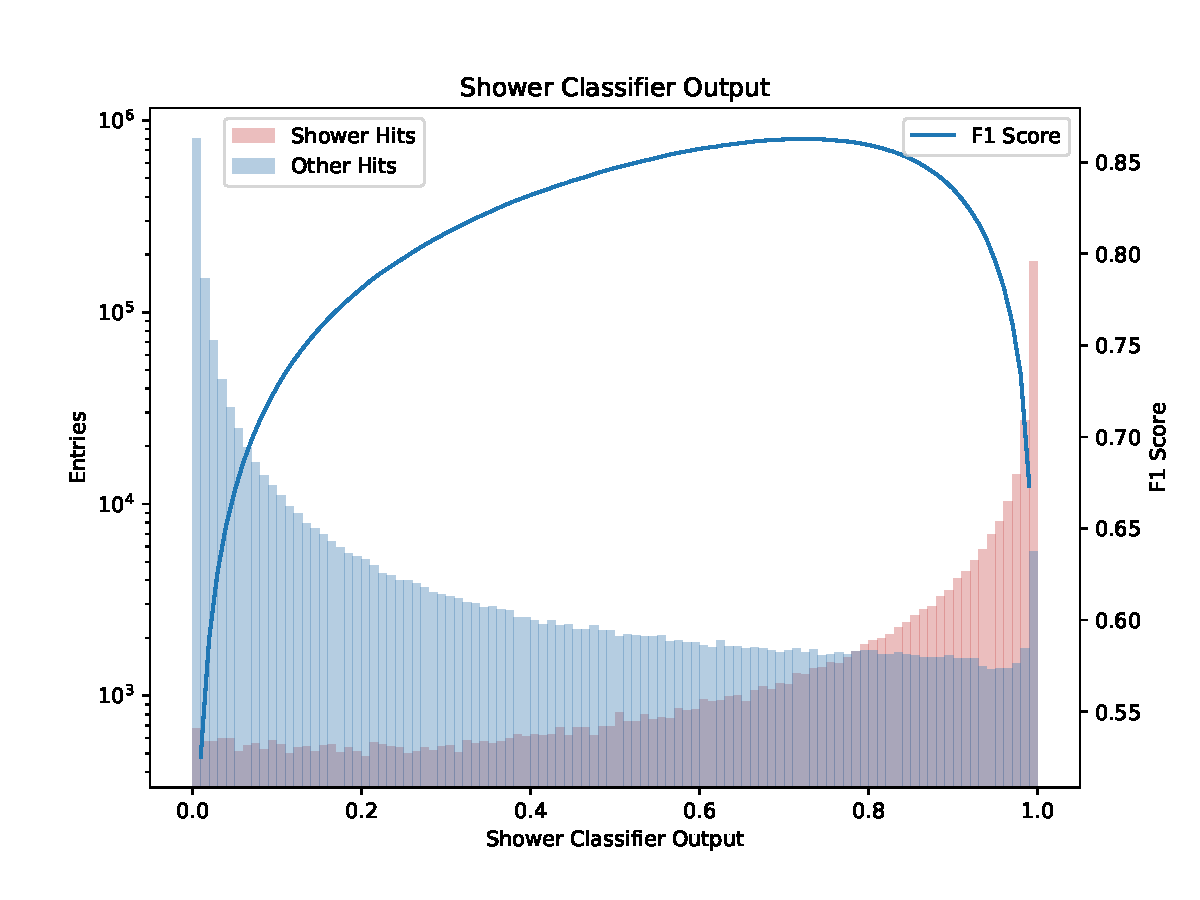
\includegraphics[width=0.9\textwidth]{figures/shower_combined.pdf} 
	\caption
	[Shower classifier output distributions.]
	{Shower classifier output distributions for true showers, and all other hits. 
	Threshold optimisation was done using the F1 score metric which is also 
	plotted.}
	\label{fig:show_output}
\end{figure}

The overall performance of the shower classifier can also be evaluated with an
receiver operating characteristic (ROC) curve\cite{Fawcett2006}. The ROC curve
shows the true positive rate vs the false positive rate for the classifier, as
the selection threshold is varied. Figure \ref{fig:show_roc} shows two ROC
curves for the shower classifier, one which is evaluated in simulation including
the space charge effect (SCE), and the other which excludes the SCE. Both curves
demonstrate that the network is capable of achieving high true positive rates,
while maintaining low false positive rates. In addition, their is a very close
agreement between the two curves, which suggests that the shower classifier is
robust to changes in the SCE model.

\begin{figure}
	\centering
	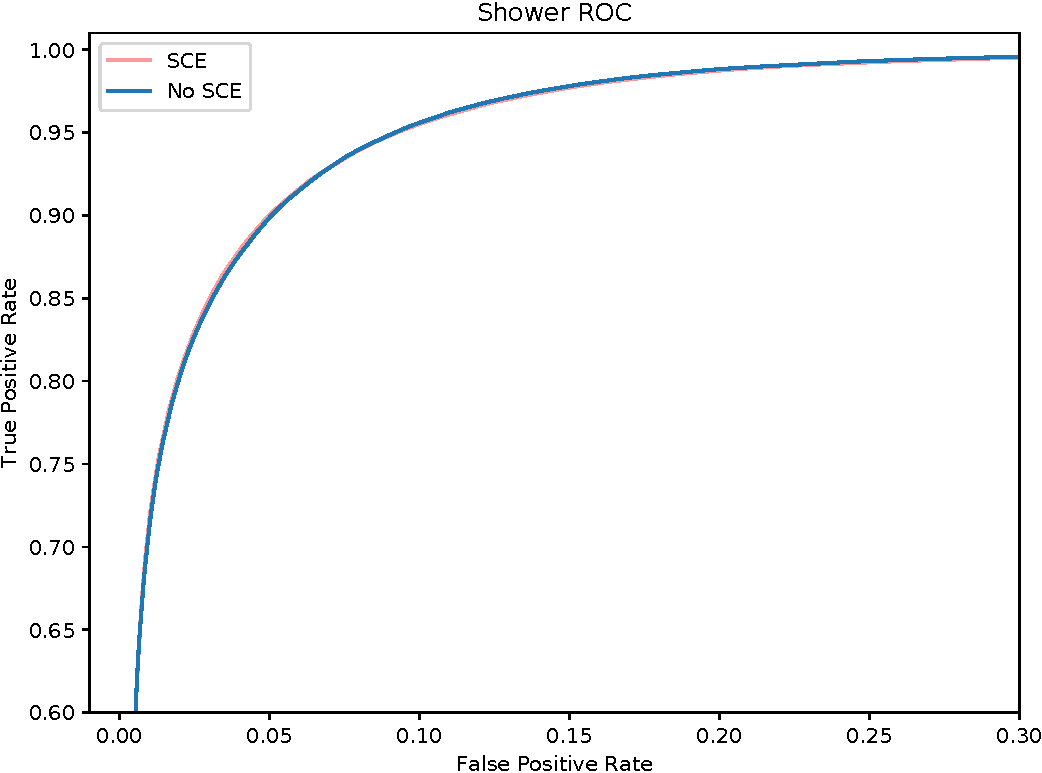
\includegraphics[width=0.9\textwidth]{figures/show_roc_comparison.pdf}
	\caption
	[ROC curve for the shower classifier.]
	{ROC curves for the shower classifier.}
	\label{fig:show_roc}
\end{figure}

\section{Validation and Performance on ProtoDUNE--SP Data} \label{cnn-perf-data}


